\section{Appendix.1 Value of Information (Two-game Chess)}
Set $P_w = 0.45$, $P_d=0.9$

\textbf{Open-loop} \\
There are 4 possible choices
\[
    \left\{\begin{array}{ccc}
        \text{\rm Policy}   &   \text{Possible cases to win} &   \text{Possibility to win}   \\
        \{B,B\}             &   \{w,w\},\{l,w,w\},\{w,l,w\}  &   P_w^2+2\cdot P_w^2(1-P_w)   \\
        \{B,T\}             &   \{w,d\},\{w,l,w\}            &   P_w P_d+P_w^2(1-P_d)        \\
        \{T,B\}             &   \{d,w\},\{l,w,w\}            &   P_d P_w+(1-P_d)\cdot P_w^2  \\
        \{T,T\}             &   \{d,d,w\}                    &   P_d^2P_w  \\
    \end{array}\right.
\]
$ J^*_{\text{\rm open-loop}}=\max \{P_w^2+2\cdot P_w^2(1-P_w),P_w P_d+P_w^2(1-P_d),P_d^2P_w\} = 42.5\% $

\textbf{Closed-loop} \\
\centerline{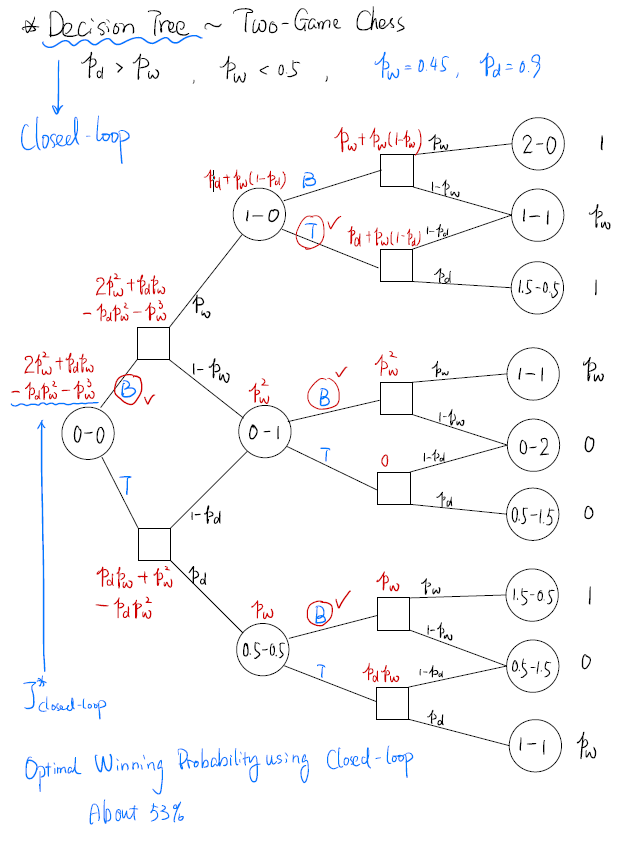
\includegraphics[width=10cm]{Lecture1/Fig3.png}}
$ J^*_{\text{\rm closed-loop}}=53\%$

\textbf{Value of information} \\
$J^*_{\textbf{\rm closed-loop}} - J^*_{\textbf{\rm open-loop}} = 10.5\%$